\documentclass[12pt]{article}
%\usepackage{mathbbold}
\usepackage{ctex}
\usepackage{amsfonts,mathrsfs,amsthm,amssymb,amsmath}
\usepackage{multirow}
\usepackage{bbding}
\usepackage{graphicx,color}
\usepackage{subfig}
\usepackage{rotating}
\usepackage[justification=justified,singlelinecheck=off]{caption}
\captionsetup[table]{name=表}
\usepackage{bm}
\usepackage{epstopdf}
\usepackage[colorlinks,linkcolor=blue,urlcolor=blue,anchorcolor=blue,citecolor=blue]{hyperref}
\usepackage[noend]{algpseudocode}
\usepackage{algorithmicx,algorithm}
\usepackage{natbib}
\usepackage{longtable,booktabs}
\usepackage{geometry}
\usepackage{CJK}
\usepackage{comment}  % 加载 comment 包
% \usepackage{minted}	  % 代码包
\usepackage{array}  % 导入 array 宏包
% \usepackage{ragged2e}  % 提供 \RaggedRight
\usepackage{tabularx}  % 导入 tabularx 宏包
\usepackage{listings}  % 插入代码
% TODO \usepackage{xeCJK} % 支持中文		依赖于 XeTeX
\usepackage{authblk}

%\usepackage{times}
%\usepackage{colortbl}
%\renewcommand{\theequation}{\thesection.\arabic{equation}}%for the form (1.1)(2.8)
\geometry{a4paper, left=2.5cm,right=2.5cm,top=2.5cm,bottom=2.5cm}

\linespread{1.4}

\renewcommand{\tablename}{\footnotesize\textbf{Table}}

%\theoremstyle{plain} \newtheorem{theorem}{Theorem}
%\theoremstyle{definition} \newtheorem{Defi}{Definition}
%\theoremstyle{remark} \newtheorem{Rem}{Remark}
%\theoremstyle{plain} \newtheorem{lemma}{Lemma}

\newtheorem{defi}{\sc Definition}[section]
\newtheorem{theorem}{\sc Theorem}[section]
\newtheorem{lemma}{\sc Lemma}[section]
\newtheorem{prop}{\sc Proposition}[section]
\newtheorem{coro}{\sc Corollary}[section]
\newtheorem{rema}{\sc Remark}[section]
%\newtheorem{exam}{\sc Example}[section]
\renewcommand{\theequation}{{\arabic{section}.\arabic{equation}}}

%the four below to generate roman number
\makeatletter
\newcommand{\rmnum}[1]{\romannumeral #1}
\newcommand{\Rmnum}[1]{\expandafter\@slowromancap\romannumeral #1@}
\newcommand{\M}{\mathcal{M}}
% 报错(Command \I already defined.LaTeX) \newcommand{\I}{\mathcal{I}}
\newcommand{\whb}{\widehat{\bm\beta}}

\makeatother

\renewcommand{\algorithmicrequire}{\textbf{Input:}}
\renewcommand{\algorithmicensure}{\textbf{Output:}}

\lstset{
    language=Matlab,      % 设置代码的语言为 Matlab
	extendedchars=true,   % 允许非 ASCII 字符
    basicstyle=\ttfamily, % 设置代码字体为等宽字体
    numbers=left,         % 显示行号
    numberstyle=\tiny,    % 行号的字体样式
    stepnumber=1,         % 行号递增的步长
    numbersep=5pt,        % 行号与代码之间的间距
    % backgroundcolor=\color{lightgray}, % 背景色
    frame=single,         % 代码框
    captionpos=b,         % 标题位置
    breaklines=true,      % 自动换行
    showstringspaces=false,  	 % 不显示字符串中的空格
    keywordstyle=\color{blue},   % 关键词样式
    commentstyle=\color{green},  % 注释样式
    stringstyle=\color{red},     % 字符串样式
	commentstyle=\color{gray},   % 设置注释的样式为灰色
	literate={\%\%}{\%\%}{2},    % 特别处理 `%%`,让它正确显示
	literate={\%}{\%}{1}      	 % 特别处理 `%` 符号,让它正确显示
}


% 报告主体部分
\begin{document}
\title{羽毛球球员表现的贝叶斯分析:\\ 多重因素下的胜率}
\date{\today}

% TODO
\author[1,2]{shenyuchen\thanks{Email: shenli24@nudt.edu.cn}}

\affil[1]{国防科技大学, 智能科学学院, 湖南, 410003}
\affil[2]{中国兵器装备集团自动化研究所有限公司智能制造事业部, 四川 绵阳, 621000}

% 作者的英文介绍 TODO


\maketitle

% 摘要
\renewcommand{\abstractname}{摘要}
\begin{abstract}
	本文主要从贝叶斯和羽毛球的发展开篇,阐述研究目标后,介绍羽毛球比赛数据的来源与预处理的数据样式。以此数据为可信基础,提取比赛表现相关的特征向量,为后续的建模奠定了基础。从模型概述、模型构建、马尔可夫链蒙特卡罗(MCMC)方法采样建立贝叶斯推理框架,实验部分展示模型获得的预测结果。最后,文章总结了研究的主要发现,探讨了模型的局限性,并对未来的研究方向进行了展望。
\end{abstract}

\textbf{关键词}: 贝叶斯;羽毛球;羽毛球世界联合会

\renewcommand{\abstractname}{Abstract}
\begin{abstract}
	This paper begins with an introduction to Bayesian inference and the development of badminton, followed by the research objectives. It then presents the source of the badminton match data and the preprocessing steps, including the data format. Using this data as a reliable foundation, feature vectors related to match performance are extracted to lay the groundwork for subsequent modeling. The paper provides an overview of the model, the construction process, and the application of the Markov Chain Monte Carlo (MCMC) method for sampling to build a Bayesian inference framework. In the experimental section, the predictive results obtained from the model are presented. Finally, the paper summarizes the main findings, discusses the limitations of the model, and offers prospects for future research directions.
\end{abstract}

\textbf{Keywords}: Bayesian; Badminton; Badminton World Federation; BWF


\section{引言(Introduction)}
\subsection{贝叶斯发展的三个阶段}
贝叶斯起源于18世纪,一个贝叶斯完整的形成简述成以下三个阶段:

①贝叶斯的发现

由英国学者托马斯·贝叶斯(T.R.Bayes,1702-1761)撰写的论文《An Essay towards solving a Problem in the Doctrine of Chances》《论有关机遇问题的求解》中,首次阐述了这一理论。在本篇论文中,贝叶斯提出通过观察新的样本数据,重新调整对某个事件的发生概率的估计。本篇论文发表于1763年,是在贝叶斯离世后的2年后,由他的朋友理查德·普赖斯(Richard Price)整理并发表出来,让世人才有机会揭开当今在人工智能领域如火如荼的真面目。

②贝叶斯定理的核心思想

如何根据先验知识(已知的数据)调整概率的预测,其数学形式如下:
\begin{equation}
	P(A|B){P(B)}={P(B|A)P(A)}
	\end{equation}
\begin{equation}
    P(A|B)=\frac{P(B|A)P(A)}{P(B)}
\end{equation}

其中:
\begin{itemize}
	\item $P(A|B)$ 是在事件 B 条件给定的情况下,事件 A 发生的概率。
	\item $P(B|A)$ 刚好与 $P(A|B)$ 相反,是在事件 A 条件给定的情况下,事件 B 发生的概率。
	\item $P(A)$、$P(B)$ 分别是事件 A 和事件 B 各自独立发生的概率。
	\end{itemize}

通过贝叶斯定理,可以将先验概率(对事件 A 的初步概率猜测)的基础之上,加上新的证据(新的样本、新的数据)相结合,得到更新后的概率(后验概率)。

③贝叶斯的发展

起初只是停留在理论层面的发展,随着计算机技术的不断发展,尤其是从20世纪以来,贝叶斯方法已经成为现代统计学、人工智能、机器学习中的核心一环。


\subsection{羽毛球的发展 \& BWF}
\begin{comment}
	简要介绍羽毛球比赛的相关背景,为什么选择使用贝叶斯推理进行分析。
\end{comment}

\begin{figure}[h]
	\centering
	\subfloat[中国的踢毽子]{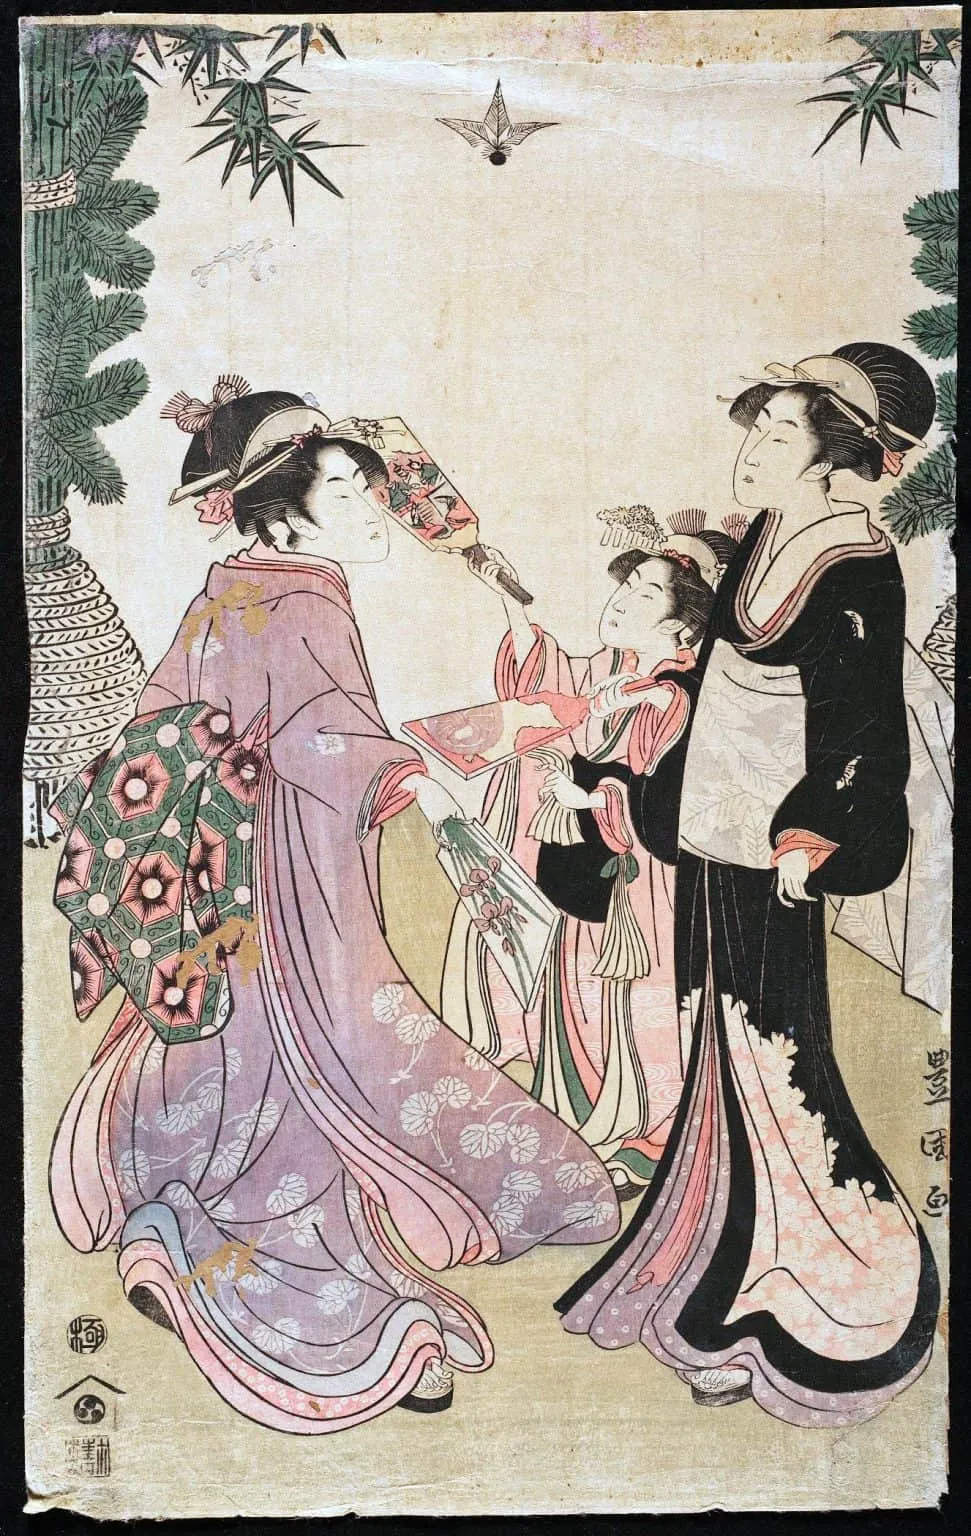
\includegraphics[width=0.48 \linewidth]{../images/history_2_ti_jian_zi}}
	\subfloat[国外打羽毛球的起源]{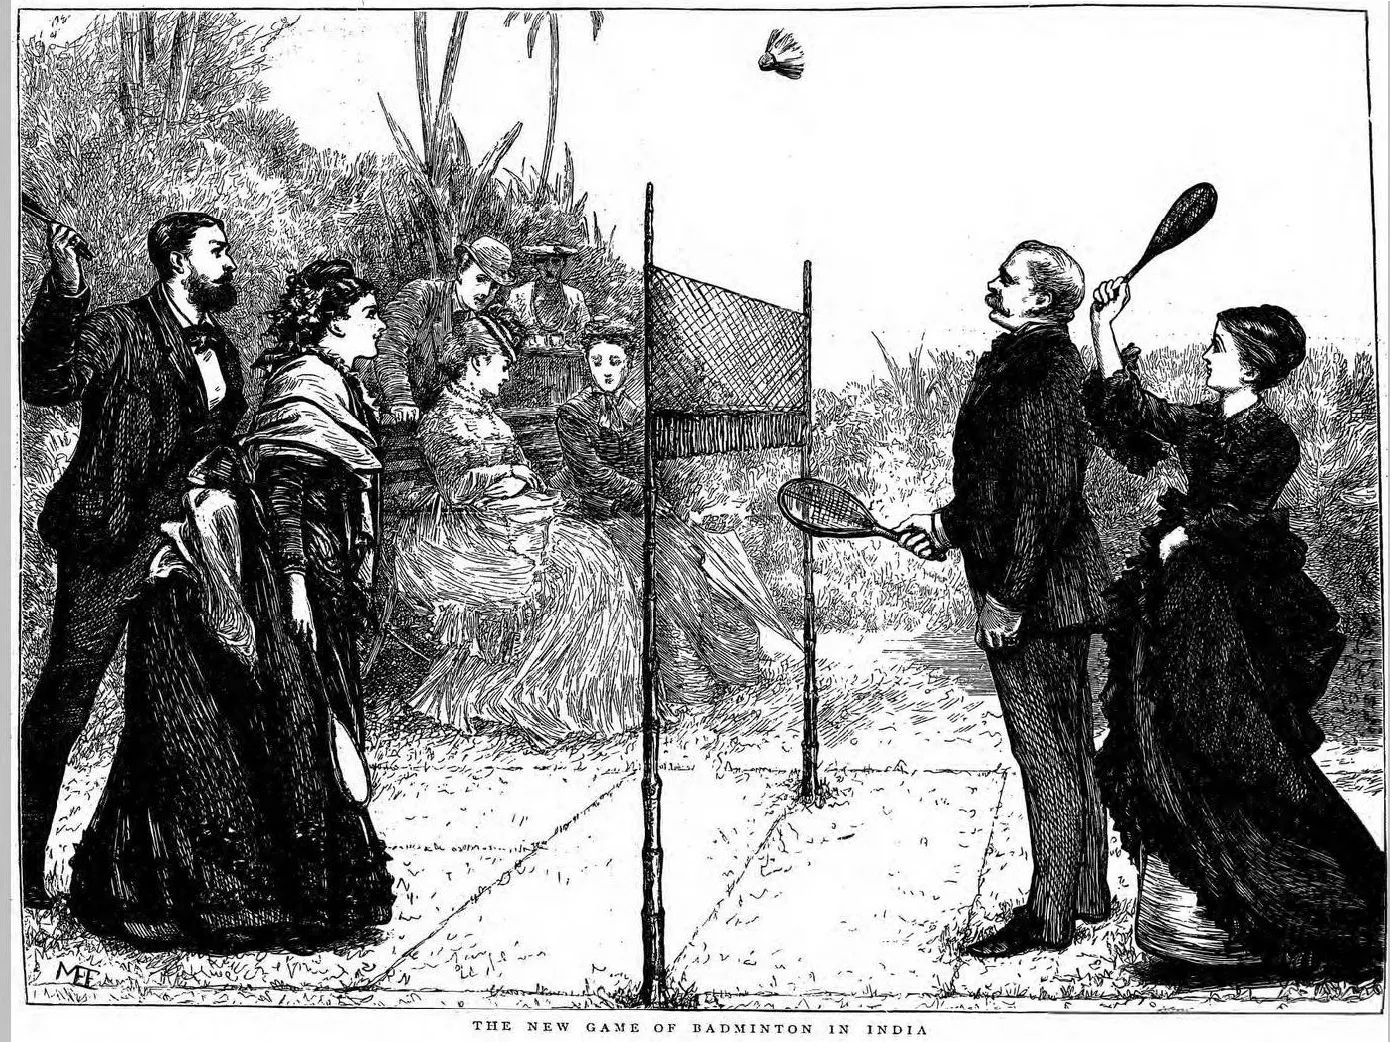
\includegraphics[width=0.48 \linewidth]{../images/history_1}}
	\caption{羽毛球的发展历史}
	\label{fig:histoys}
\end{figure}


随着体育事业的不断发展,羽毛球的体育赛事逐渐进入人们的视野。
在中国,早在 2000 年前就有人玩一种叫做“踢毽子”的游戏。这个游戏通过用脚相互踢毽子,不仅是一种娱乐活动,还能锻炼人体的灵活性和协调性。(如图 $\ref{fig:histoys}$ 所示)

1877年,英国巴斯羽毛球俱乐部(Bath Badminton Club)在英国巴斯(Bath)首次制定了羽毛球的标准规则,这些规则包括场地尺寸、网高、比赛礼仪和打法等,为羽毛球运动提供了标准和依据,成为现代羽毛球的正式起源。
1893年,由英格兰羽毛球协会(Badminton Association of England)发布,并成为现代羽毛球运动的基础。
1934年,国际羽毛球联合会成立,当时称为 International Badminton Federation(IBF)。
1992年,在巴塞罗那夏季奥运会,羽毛球首次成为正式的奥运项目。
2006年,IBF 更名为羽毛球世界联合会 World Badminton Championships(BWF)\cite{bwf2024website}。BWF 的总部在马来西亚吉隆坡,目前的成员国已经超过200+个国家。\cite{historybadminton2024website}


\subsection{研究目标}
\begin{comment}
	阐述你希望通过贝叶斯推理预测比赛结果,探索相关因素。
\end{comment}
羽毛球运动分为男子单打、女子单打、男子双打、女子双打、男女混双,本文的研究目标主要是针对,中国运动员男子单打选手,石宇奇的比赛数据(主赛事总得分、最大连续得分、赛点次数)进行预处理,并通过是对其胜率进行贝叶斯模型构建、推理、马尔可夫链蒙特卡罗(MCMC)方法采样,预测其相同比赛参数下不同数据比赛胜利的概率。


\section{数据收集与预处理(Data Collection \& Preprocessing)}
\subsection{数据来源}
Badminton World Federation 简称 \cite{bwf2024website},是羽毛球运动的全球管理机构,负责组织和管理国际羽毛球赛事,包括世界羽毛球锦标赛和世界羽毛球巡回赛等,提供关于羽毛球比赛的最新动态、赛事结果、运动员信息以及相关技术分析等内容。


\subsection{预处理数据}

以最新的2024年第47周的 \cite{shiYuqi2024website} 官方数据为例,可整理得以下表格数据,见表 $\ref{fig:LI-NING China Masters 2024}$ 。
\begin{table}[h!]
	\centering
	\begin{tabularx}{\textwidth}{|l|X|X|X|X|X|}
	\hline
	\textbf{Opponent} & \textbf{Total Scores} & \textbf{Rounds Number} & \textbf{Max Consecutive Points} & \textbf{Game Points} & \textbf{Victory Labels} \\
	\hline
	Jonatan CHRISTIE & 33 & 2 & 4 & 0 & 0 \\
	Kunlavut VITIDSARN & 42 & 2 & 6 & 4 & 1 \\
	Chico Aura DWI WARDOYO & 42 & 2 & 7 & 3 & 1 \\
	Chia Hao LEE & 42 & 2 & 7 & 5 & 1 \\
	\hline
	\end{tabularx}
	\caption{LI-NING China Masters 2024 Results}
	\label{fig:LI-NING China Masters 2024}
\end{table}


\section{贝叶斯推理模型(Bayesian Inference Model)}

\subsection{模型概述}
\begin{comment}
	解释贝叶斯定理和你如何应用它进行比赛结果预测。
	详细描述模型的构建过程,包括先验概率、似然函数和后验概率的计算。
	\end{comment}

对于羽毛球球员在多重因素下的胜率这个问题下,我们的任务就是:使用已有的比赛参数(比如主赛事总得分、对局轮次、最大连续得分、赛点次数、胜负情况、等等)的数据,来预测比赛参数相同但是数据不同时,对该运动员在未来比赛中的胜利概率预测。
贝叶斯推理可以帮助我们通过已有的比赛数据(样本数据)来更新模型参数的后验分布,从而做出预测。在本文中,我们将采用 MCMC 方法生成参数的样本,近似计算后验分布,进而计算运动员的胜利概率。

\subsection{贝叶斯推理模型框架}
根据羽毛球世界联合会的官网我们可以获取运动员相关的比赛数据,我们可以使用一个简单的二项分布来描述每场比赛的结果(胜利或者失败),根据贝叶斯定理来更新模型参数的后验分布:

\begin{equation}P(\theta|X)=\frac{P(X|\theta)P(\theta)}{P(X)}\end{equation}

其中:
\begin{itemize}
	\item $P(\theta|X)$ 是后验概率(给定数据 X,参数 $\theta$ 的概率分布)。
	\item $P(X|\theta)$ 是似然函数(给定参数 $\theta$,数据 X 的概率分布)。
	\item $P(\theta)$ 是先验概率(参数 $\theta$ 的先验分布)。
	\item $P(X)$ 是边际似然,通常作为归一化常数。
	\end{itemize}


在比赛预测中,假设每一个比赛的胜负由一个伯努利分布模型来描述:
\begin{equation}
	P(\mathrm{victory}=1|\theta)=\sigma(\theta)
	\end{equation}

其中 $\sigma(\theta)$ 是一个激活函数(比如:sigmoid)将参数 $\theta$ 映射到 [0,1] 范围,表示胜利的概率。

\begin{equation}
	\sigma(x)=\frac{1}{1+e^{-x}}
\end{equation}


\subsection{模型构建}
使用的数据包括如下五个部分:
\begin{itemize}
	\item 主赛事总得分 (\text{total\_scores}):主赛事总得分    运动员在本场主赛事中的总比分。注意每一场不一定是在21分时结束,可能出现延长比赛的情况,同时,也可能发生对手或本人因伤病或其他原因弃赛的情况,这些都将影响最终的总比分。注意,延长赛:如果一局比赛的比分进入到21分之后,两位选手或队伍的得分相差不到两分(例如20-20),这时比赛会进入加赛,直到一方领先2分为止。这种加赛通常没有上限,直到有一方完成领先。
	\item 对局轮次 (\text{rounds\_number}):一般是三局两胜制,也不排除五局三胜,每场主赛事的规则由活动方规定。
	\item 最大连续得分 (\text{max\_consecutive\_points}):与不同运动员对赛时的单次对局时的最大连续得分的数据。
	\item 赛点次数 (\text{game\_points}):羽毛球中的“赛点”指的是比赛中一方可以赢得比赛的关键时刻,即如果该方赢得当前的分数,便会最终获胜。赛点次数是与不同运动员对赛时的单次对局时的赛点次数。
	\item 胜负情况 (\text{victory\_labels}):与不同运动员对赛时的单次对局时的胜负情况。
\end{itemize}

为了方便后文的表述,我们在此约定,一个运动员的实力值由对局轮次、大连续得分、赛点次数三个部分构成,且在本文中各自的权重无偏好,即其表达式:实力值 = 对局轮次 + 最大连续得分 + 赛点次数。


我们的分类模型采用线性回归模型,用于表示数据与结果之间的关系。假设我们需要根据历史的比赛统计数据预测比赛的胜利与否(即胜负二分类问题),我们可做出如下定义:
\begin{itemize}
	\item $y_{i}$ 是第 i 场比赛的胜利情况(1表示胜利,0表示失败)。
	\item $x_{i}$ 是第 i 场比赛的特征向量,其中:
	\begin{itemize}
		\item $x_{i1}$ 是主赛事总得分
		\item $x_{i2}$ 是最大连续得分
		\item $x_{i3}$ 是赛点次数
	\end{itemize}
\end{itemize}
构造以下的逻辑回归模型来描述比赛结果:
\begin{equation}
    P(y_i=1|x_i)=\frac{1}{1+\exp(-(\beta_0+\beta_1x_{i1}+\beta_2x_{i2}+\beta_3x_{i3}))}
\end{equation}
这里,$\beta_0,\beta_1,\beta_2,\beta_3$ 是模型的参数,是需要通过历史的数据进行估计的。

\subsection{贝叶斯推理}
根据贝叶斯定理,给定数据 $D=\{(x_1,y_1),(x_2,y_2),\ldots,(x_N,y_N)\}$,我们希望计算参数 $\theta=(\beta_0,\beta_1,\beta_2,\beta_3)$ 的后验分布:
\begin{equation}
    P(\theta|D)\propto P(D|\theta)P(\theta)
\end{equation}
其中:
\begin{itemize}
	\item $P(D|\theta)$ 是似然函数,表示在给定参数 $\theta$ 的情况下,数据 D 出现的概率。
	\item $P(\theta)$ 是先验分布,表示我们对参数 $\theta$ 的先验知识。
\end{itemize}


\subsection{马尔可夫链蒙特卡罗(MCMC)方法采样}
使用马尔可夫链蒙特卡罗(MCMC)方法来从后验分布 $P(\theta|D)$ 中进行采样。
它是一种通过构造一个马尔可夫链来模拟目标分布的抽样方法。MCMC 方法可以应用于大部分贝叶斯模型,特别是当模型较复杂,无法直接计算后验概率时。MCMC 可以帮助我们通过采样来近似后验分布,此处我们使用 Metropolis-Hastings 算法来生成后验分布的样本。

步骤1:我们需要计算每个参数组合的后验概率。对于逻辑回归模型,后验概率为:
\begin{equation}
    P(\theta|D)\propto\prod_{i=1}^N\left[P(y_i|x_i;\theta)\right]P(\theta)
\end{equation}
其中,$P(y_i|x_i;\theta)$ 是逻辑回归模型的似然函数,即:
\begin{equation}
	\resizebox{\textwidth}{!}{$
	P(y_i|x_i;\theta)=\left[\frac{1}{1+\exp(-(\beta_0+\beta_1x_{i1}+\beta_2x_{i2}+\beta_3x_{i3}))}\right]^{y_i}\left[1-\frac{1}{1+\exp(-(\beta_0+\beta_1x_{i1}+\beta_2x_{i2}+\beta_3x_{i3}))}\right]^{1-y_i}
	$}
\end{equation}

步骤2:使用 Metropolis-Hastings 算法,步骤如下:
\begin{enumerate}
	\item 从样本数据中随机选择初始参数 $\theta^{(0)}=(\beta_0,\beta_1,\beta_2,\beta_3)$。
	\item 通过跳跃选择新的参数(候选参数) $\theta^{\prime}$ 。
	\item 计算接受概率 $\alpha(\theta,\theta^{\prime})$,并决定是否接受 $\theta^{\prime}$:
	\begin{equation}
		\alpha(\theta,\theta^{\prime})=\min\left(1,\frac{P(D|\theta^{\prime})P(\theta^{\prime})}{P(D|\theta)P(\theta)}\right)
	\end{equation}
	\item 如果接受 $\theta^{\prime}$,则 $\theta^{(t+1)}=\theta^{\prime}$,否则保持 $\theta^{(t+1)}=\theta^{(t)}$ 。
	\item 重复以上过程,直到收敛。
\end{enumerate}


\section{实验与结果(Experiment \& Results)}
一旦我们得到了后验分布,我们可以通过计算预测概率来预测未来比赛的胜负:
\begin{equation}
    P(y_{new}=1|x_{new})=\frac{1}{1+\exp(-(\beta_0+\beta_1x_{new1}+\beta_2x_{new2}+\beta_3x_{new3}))}
\end{equation}
其中,$x_{new}$ 是未来比赛的特征。

步骤1:通过三场主赛事,九场对局轮次的比赛数据,详见表格 $\ref{fig:three main tournaments}$。

\renewcommand{\arraystretch}{1.2} % 调整行间距
\begin{table}[h!]
\centering
\scriptsize % 缩小字体,防止超出边框
\setlength{\tabcolsep}{3pt} % 减少列间距
\begin{tabular}{|p{3.5cm}|p{3.8cm}|p{1.2cm}|p{1.2cm}|p{1.8cm}|p{1.2cm}|p{1.2cm}|}
\hline
\textbf{main tournaments} & \textbf{opponents} & \textbf{total scores} & \textbf{rounds number} & \textbf{max consecutive points} & \textbf{game points} & \textbf{victory labels} \\ \hline

\multirow{4}{3.5cm}{LI-NING China Masters 2024} 
& Jonatan CHRISTIE          & 33 & 2 & 4  & 0 & 0 \\ \cline{2-7}
& Kunlavut VITIDSARN        & 42 & 2 & 6  & 4 & 1 \\ \cline{2-7}
& Chico Aura DWI WARDOVO    & 42 & 2 & 7  & 3 & 1 \\ \cline{2-7}
& Chia Hao LEE              & 42 & 2 & 7  & 5 & 1 \\ \hline

\multirow{2}{3.5cm}{VICTOR China Open 2024} 
& Anthony Sinisuka GINTING  & 19 & 2 & 4  & 0 & 0 \\ \cline{2-7}
& Kantaphon WANGCHAROEN     & 24 & 2 & 10 & 3 & 1 \\ \hline

\multirow{3}{3.5cm}{Korea Open 2024} 
& LEE Cheuk Yiu             & 28 & 2 & 4  & 0 & 0 \\ \cline{2-7}
& NG Ka Long Angus          & 42 & 2 & 5  & 2 & 1 \\ \cline{2-7}
& SON Wan Ho                & 42 & 2 & 6  & 3 & 1 \\ \hline

\end{tabular}
\caption{LI-NING China Masters 2024、VICTOR China Open 2024、Korea Open 2024 三场主赛事的官方比赛数据}
\label{fig:three main tournaments}
\end{table}

步骤2:我们使用工具进行仿真模拟,横轴(Match Number)表示相应场次,纵轴(Predicted Victory Probability)表示相应场次的赢得比赛预测概率的结果,详见图片 $\ref{fig:probability results}$。

\begin{figure}[h]
	\centering
	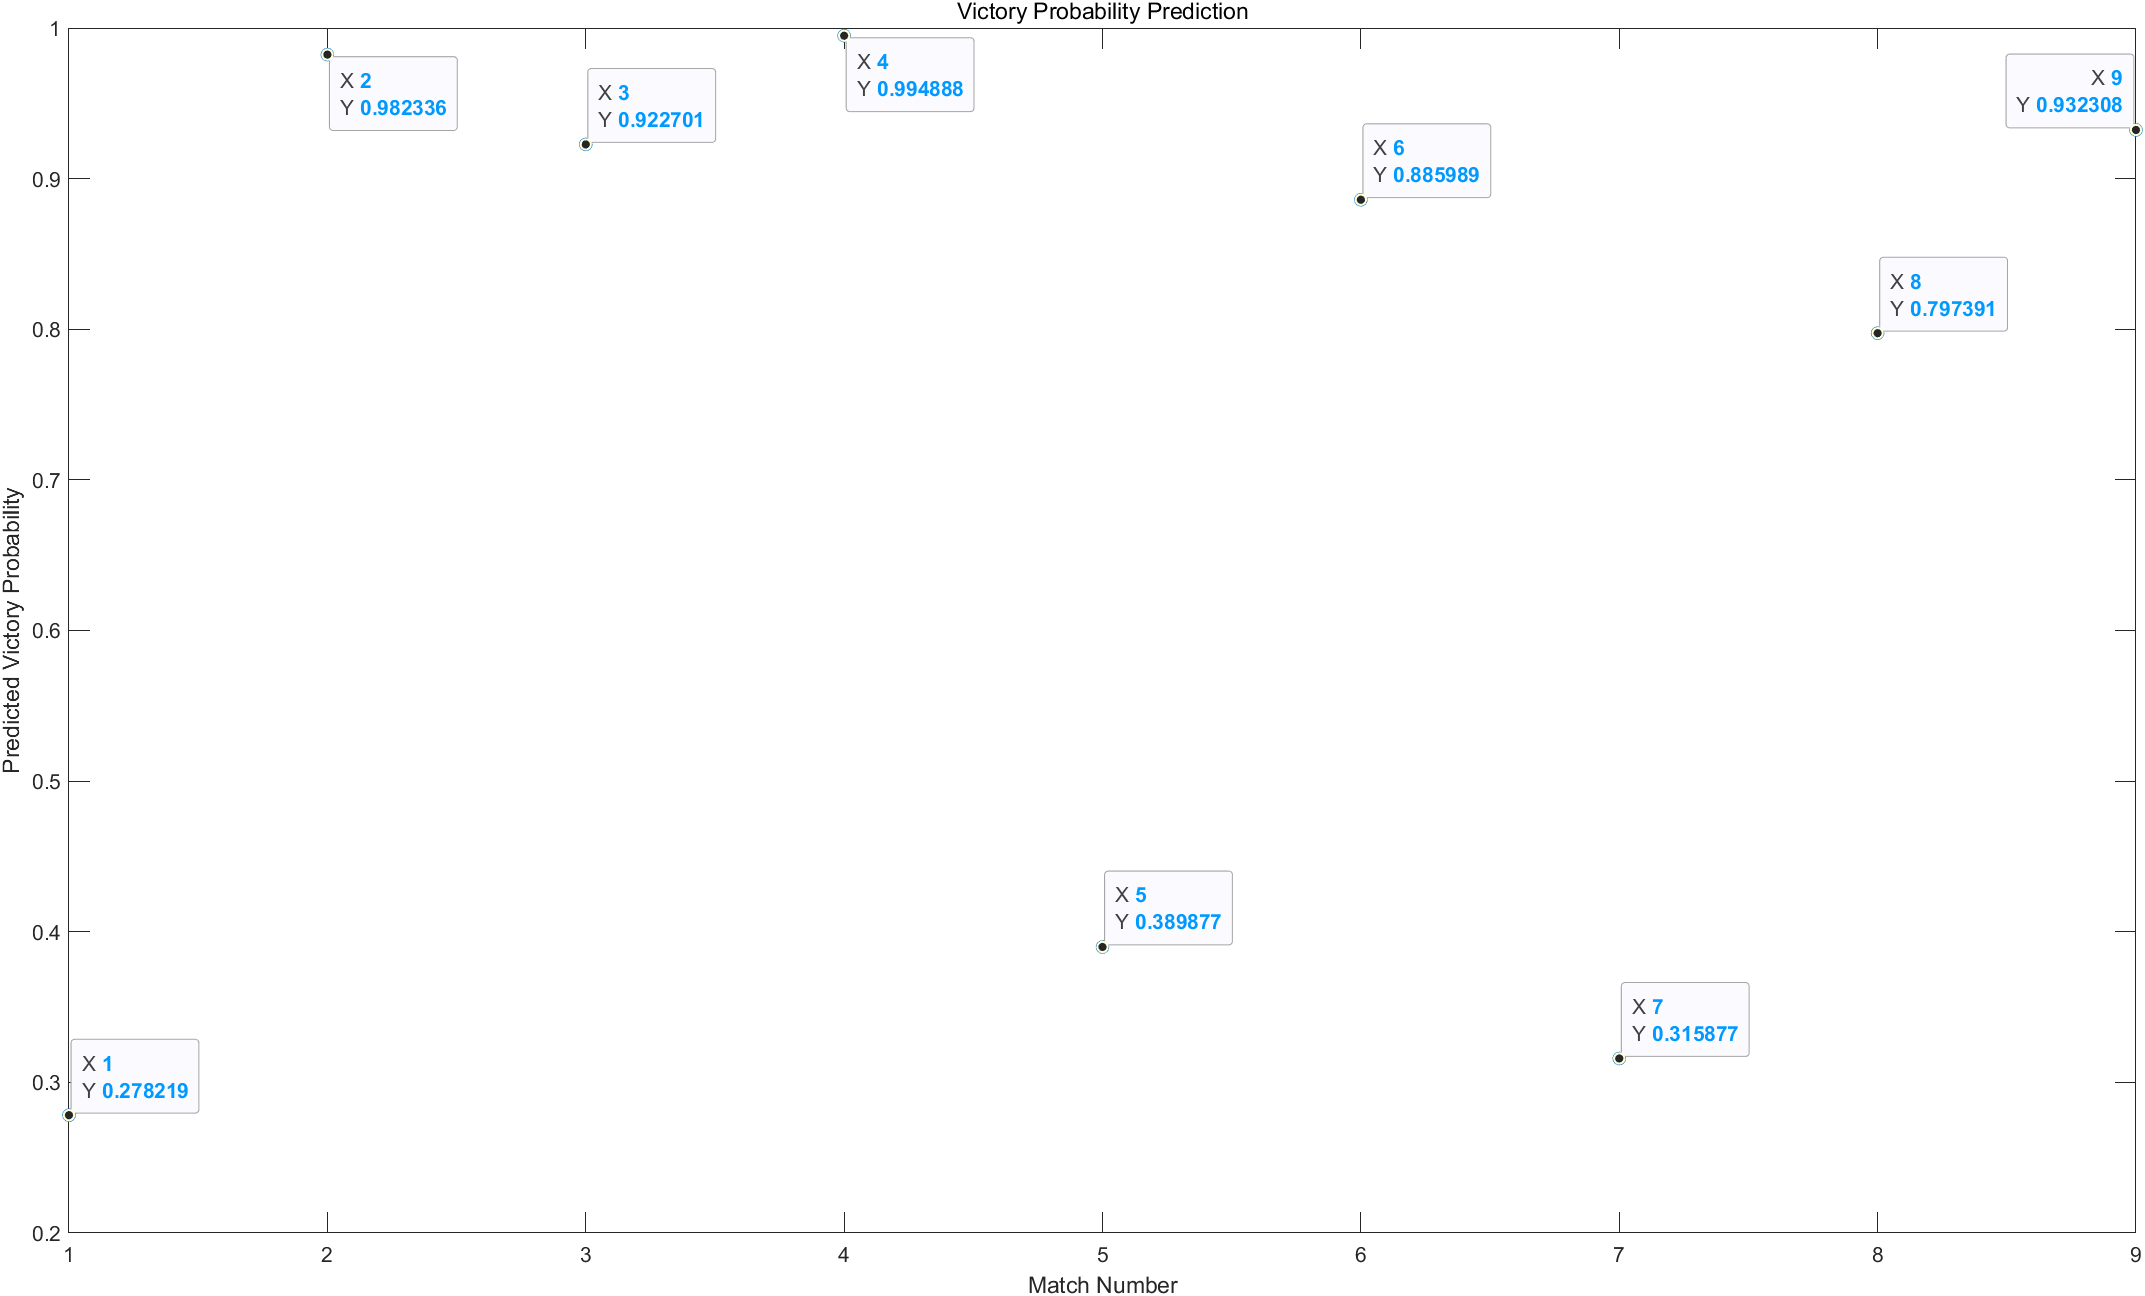
\includegraphics[width=0.8\textwidth]{../images/probability results}
	\caption{根据历史比赛数据,预测相同比赛参数下不同数据的比赛胜利的概率}
	\label{fig:probability results}
\end{figure}
例如:

对于第 5 场比赛( X=5 ),对其胜利预测的概率为 0.389877( Y=0.389877 ),与数据中的结果比较符合,最终对局结果确实输掉了( victory labels=0 )。

对于第 4 场比赛( X=4 ),对其胜利预测的概率为 0.994888( Y=0.994888 ),也与数据中的结果符合。此时最大连续得分数为7( max consecutive points=7 ),且赛点次数为 5( game points=5 ),最终拿下本次对局( victory labels=1 )。


\section{总结与展望(Conclusion \& Prospect)}
对于本模型,可以对一些实力值参数进行加权,比如最大连续得分比赛点次数和对局轮次肯定更重要。如果一个运动员在一场比赛中连续得分,那么他的实力值肯定是更大一些的,这也是符合我们直觉的。当然,这得通过实验验证,也有可能是对手的故意丢分,通过以自己最小的体力消耗,前期调动对手较大的体力值,从而在比赛前期保存自己的体力,为后期赢得比赛最终胜利所采取的比赛策略。

除了上述三种实力值,可能影响预测结果的因素还有其他可以考虑的信息,比如球员的身体状况、比赛场地、排名、赛季表现、年龄、比赛场地类型、对手的水平等,而且对于同一个对手也可以试试:
\begin{itemize}
	\item 通过分析运动员本人与同一个人多次对战的数据,进而预测出运动员本人下一次与同一个人对战胜利概率。
	\item 还可以通过分析对手与不同其他运动员对战的数据,分析出最优战胜该对手的运动员推荐,以较低的代价赢得比赛。
\end{itemize}

本文也只分析了男子单打、还可以从女子单打、男子双打、女子双打、男女混双,这四个比赛模式分析。

同时贝叶斯分类模型,还可以尝试使用其他机器学习方法(如支持向量机、决策树、随机森林等)进行对比分析。


% 参考文献
\begin{thebibliography}{100}
	\expandafter\ifx\csname natexlab\endcsname\relax\def\natexlab#1{#1}\fi
	\expandafter\ifx\csname url\endcsname\relax
	\def\url#1{\texttt{#1}}\fi
	\expandafter\ifx\csname urlprefix\endcsname\relax\def\urlprefix{URL }\fi

\bibitem[{Wang and Chu(2021)}]{wang2021bayesian}
Wang, Z. and Chu, X., 2021. 贝叶斯决策理论对复杂运动决策中运动预期的启发——以网球和足球为例. \textit{Psychological Science Progress}, \textbf{7}, 1300–1312.
\bibitem[{Percy(2015)}]{percy2015mathematical} 
D. F. Percy.A Mathematical Analysis of Badminton Scoring Systems[J].\textit{Operational Research Applied to Sports}, 2015:181-200.
\bibitem[{Niu(2012)}]{niu2012bayesian}
Niu, Z., 2012. 基于贝叶斯网络的NBA比分预测和球员能力评估模型. \textit{Master's Thesis}, Huazhong University of Science and Technology.


\bibitem[{BWF(2024)}]{bwf2024website}
BWF, 2024. BWF Badminton (羽毛球世界联合会官网). Available at: \url{https://bwfbadminton.com/zh-cn/}. Accessed on: December 17, 2024.
\bibitem[{History Of Badminton(2024)}]{historybadminton2024website}
Strings and Paddles, 2024. The History of Badminton. Available at: \url{https://stringsandpaddles.com/the-history-of-badminton/}. Accessed on: December 17, 2024.
\bibitem[{ShiYuQi in LI-NING China Masters(2024)}]{shiYuqi2024website}
BWFBadminton, 2024. Shi Yuqi – LI-NING China Masters 2024. Available at: \url{https://bwfbadminton.com/zh-cn/player/57945/shi-yu-qi/}. Accessed on: December 17, 2024.

\end{thebibliography}

\appendix
\section{附录:$table\_datas\_demo\_en.m$}
使用预处理后的数据,将主赛事名称(main tournaments)、单次对局中的对手名(opponents)、主赛事总得分 (total scores)、对局轮次 (rounds number)、最大连续得分 (max consecutive points)、赛点次数 (game points)、胜负情况 (victory labels)数据保存在 $ShiYuQi\_table\_datas.mat$ 文件中,供其他文件读取使用。

\lstinputlisting[language=Matlab]{../code/table_datas_demo_en.m}


\section{附录:$bayesian\_predictive\_model\_en.m$}
通过读取预处理的数据 $ShiYuQi\_table\_datas.mat$ 构造贝叶斯推理模型,预测中国运动员选手石宇奇,在相同比赛参数下不同数据的比赛胜利的概率,并绘制出横坐标为比赛场次纵坐标对应胜利的预测概率。

\lstinputlisting[language=Matlab]{../code/bayesian_predictive_model_en.m}


\end{document}


